\begin{frame}{Neue Wechselwirkung}
\begin{itemize}
	\setlength\itemsep{1em}
	\item Neue $U(1)$-Symmetrie mit Eichboson $Z'$ \cite{InColour}
	\item Unter der neuen Wechselwirkung geladene Teilchen:
	\begin{itemize}
		\item Leptonen der zweiten und dritten Generation
		\item Neue Quarks
		\item Dunkle Materie \cite{Z}
	\end{itemize}
	\item Ein paar Worte zu $L_\mu-L_\tau$.
\end{itemize}
\end{frame}

\begin{frame}{Neue Wechselwirkung}
\framesubtitle{Kopplung der neuen Quarks an die SM-Quarks}
\begin{figure}
	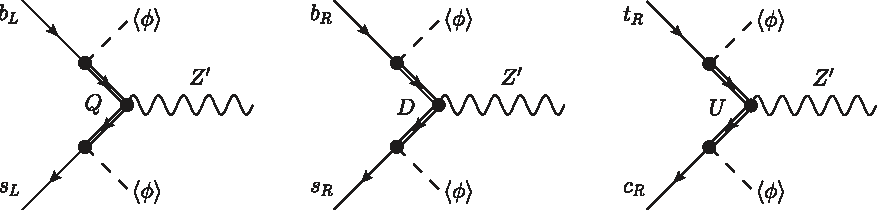
\includegraphics[width=\textwidth]{Bilder/NeueQuarks.pdf}
	\caption{Wechselwirkung von SM-Quarks mit dem Eichboson $Z'$ (aus \cite{InColour})}
\end{figure}
\end{frame}

\begin{frame}{Neue Wechselwirkung}
\framesubtitle{Loop-Diagramm zur Streuung am Atomkern}
\begin{minipage}{.25\textwidth}
%	\begin{figure}[H]
		\resizebox{1.4\textwidth}{!}{
			\begin{tikzpicture}
\tikzstyle{centerArrow}=[decoration={
	markings,
	mark=at position 0.5 with {\fill (2pt,0)--(-2pt,2.31pt)--(-2pt,-2.31pt)--cycle;}}]

\begin{scope}[xshift=6cm,yshift=5cm]
\def\xmove{2}
\def\ymove{1.25}
\def\centerShift{2cm}
\def\centerCircle{1cm}
\def\centerSize{0.05cm}
\coordinate (tCenter1) at (0,0);
\coordinate (tCenter2) at (0,-\centerShift);
\coordinate (tCenter3) at (0,-\centerShift-\centerCircle);
\coordinate (tCenter4) at (0,-\centerShift-\centerCircle-\centerShift);

\node (upperLeft) at (-\xmove,\ymove) {$\chi$};
\node (upperRight) at (\xmove,\ymove) {$\chi$};
\node (lowerLeft) at (-\xmove,-\centerShift-\centerCircle-\centerShift-\ymove cm) {$N$};
\node (lowerRight) at (\xmove,-\centerShift-\centerCircle-\centerShift-\ymove cm) {$N$};

\draw [centerArrow,postaction={decorate}]  (upperLeft) -- (tCenter1) ;
\draw [centerArrow,postaction={decorate}]  (tCenter1) -- (upperRight) ;
\draw [centerArrow,postaction={decorate}]  (lowerLeft) -- (tCenter4) ;
\draw [centerArrow,postaction={decorate}]  (tCenter4) -- (lowerRight) ;
\draw [decoration={snake, segment length=1.5mm, amplitude=0.5mm},decorate] (tCenter1) -- (tCenter2) ;
\node at (0.5,-\centerShift/2) {$Z'$};
\draw [
        decoration={markings, mark=at position 0.5 with {\fill (2pt,0)--(-2pt,2.31pt)--(-2pt,-2.31pt)--cycle;}, mark=at position 1 with {\fill (2pt,0)--(-2pt,2.31pt)--(-2pt,-2.31pt)--cycle;}},
        postaction={decorate}
] ([yshift=.5cm]tCenter3) ellipse(.45 and 0.5);
\node at ([yshift=-\centerCircle/2,xshift=0.75cm]tCenter2) {$l$};
\node at ([yshift=-\centerCircle/2,xshift=-0.75cm]tCenter2) {$l$};
\draw [decoration={snake, segment length=1.5mm, amplitude=0.5mm},decorate] (tCenter3) -- (tCenter4) ;
\node at (0.5,-\centerShift/2-\centerCircle-\centerShift) {$\gamma$};
\end{scope}
\end{tikzpicture}
		}
		%		\captionsetup{width=\textwidth}
%		\caption{Loop-Wechselwirkung zur Streuung DM am Atomkern.}
%	\end{figure}
\end{minipage}
\hfill
\begin{minipage}{.7\textwidth}
	Wirkungsquerschnitt ohne Impulsübertrag:
	\[ \sigma_\text{0,loop} = \frac{\mu_{A\chi}^2}{A^2\pi}\left(\frac{\alpha_{em}Z}{3\pi}\ \frac{g'^2q_\chi q_l}{m_{Z'}^2}\log\left(\frac{m_\mu^2}{m_\tau^2}\right)\right)^2 \]
\end{minipage}
\end{frame}

\begin{frame}{Neue Wechselwirkung}
\framesubtitle{Beschränkung der Parameter}
Seltene $B$-Zerfälle:
	\[ \SI{540}{\giga\electronvolt}\lessapprox\frac{m_{Z'}}{g'}\lessapprox\SI{4.9}{\tera\electronvolt} \]
Relic Density:
	\[ m_{Z'}\approx 2m_\chi \]
Direct Detection $(q_\chi=q_l)$:
	\[ \SI{10}{\giga\electronvolt}\lessapprox m_{Z'} \lessapprox\SI{46}{\giga\electronvolt} \]
	\[ \SI{2e-3}{}\lessapprox g' \lessapprox\SI{e-2}{} \]
\end{frame}